\tikzset{every picture/.style={line width=0.75pt}} %set default line width to 0.75pt        

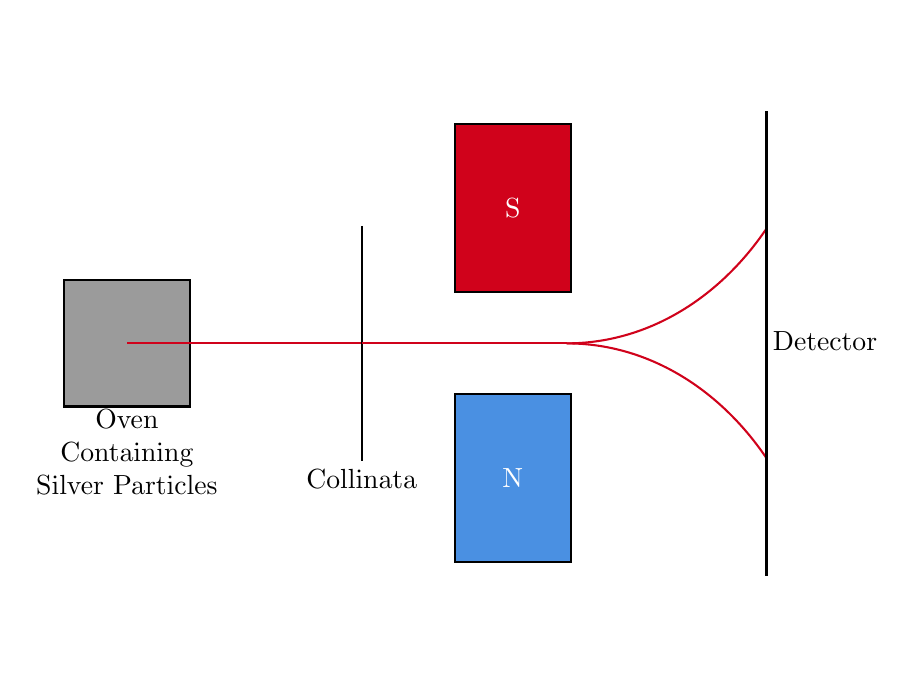
\begin{tikzpicture}[x=0.75pt,y=0.75pt,yscale=-.8,xscale=.8]
%uncomment if require: \path (0,375); %set diagram left start at 0, and has height of 375

%Shape: Square [id:dp14421103605944618] 
\draw  [fill={rgb, 255:red, 155; green, 155; blue, 155 }  ,fill opacity=1 ] (100,128) -- (176,128) -- (176,204) -- (100,204) -- cycle ;
%Straight Lines [id:da6727148484422872] 
\draw [color={rgb, 255:red, 208; green, 2; blue, 27 }  ,draw opacity=1 ]   (279.42,166) -- (138,166) ;
%Straight Lines [id:da8380240359625067] 
\draw    (279.42,95.29) -- (279.42,236.71) ;
%Shape: Rectangle [id:dp32874348023480093] 
\draw  [fill={rgb, 255:red, 208; green, 2; blue, 27 }  ,fill opacity=1 ] (335.42,34) -- (405.42,34) -- (405.42,135.29) -- (335.42,135.29) -- cycle ;
%Shape: Rectangle [id:dp31052784363324215] 
\draw  [fill={rgb, 255:red, 74; green, 144; blue, 226 }  ,fill opacity=1 ] (335.42,196.29) -- (405.42,196.29) -- (405.42,297.58) -- (335.42,297.58) -- cycle ;
%Straight Lines [id:da09102819630459058] 
\draw [color={rgb, 255:red, 208; green, 2; blue, 27 }  ,draw opacity=1 ]   (402.84,166) -- (279.42,166) ;
%Shape: Arc [id:dp14380617240917248] 
\draw  [draw opacity=0] (402.84,166) .. controls (402.84,166) and (402.84,166) .. (402.84,166) .. controls (451.32,166) and (494.63,192.92) .. (523.21,235.14) -- (402.84,355.5) -- cycle ; \draw  [color={rgb, 255:red, 208; green, 2; blue, 27 }  ,draw opacity=1 ] (402.84,166) .. controls (402.84,166) and (402.84,166) .. (402.84,166) .. controls (451.32,166) and (494.63,192.92) .. (523.21,235.14) ;  
%Shape: Arc [id:dp018293912875773533] 
\draw  [draw opacity=0] (402.84,166) .. controls (402.84,166) and (402.84,166) .. (402.84,166) .. controls (451.32,166) and (494.63,139.08) .. (523.21,96.86) -- (402.84,-23.5) -- cycle ; \draw  [color={rgb, 255:red, 208; green, 2; blue, 27 }  ,draw opacity=1 ] (402.84,166) .. controls (402.84,166) and (402.84,166) .. (402.84,166) .. controls (451.32,166) and (494.63,139.08) .. (523.21,96.86) ;  
%Straight Lines [id:da21129461638831382] 
\draw    (523.21,164.43) -- (523.21,305.85) ;
%Straight Lines [id:da4601124961028422] 
\draw    (523.21,26.15) -- (523.21,167.57) ;

% Text Node
\draw (138,204) node [anchor=north] [inner sep=0.75pt]   [align=left] {\begin{minipage}[lt]{70.19pt}\setlength\topsep{0pt}
\begin{center}
Oven \\Containing \\Silver Particles
\end{center}

\end{minipage}};
% Text Node
\draw (279.42,239.71) node [anchor=north] [inner sep=0.75pt]   [align=left] {\begin{minipage}[lt]{42.43pt}\setlength\topsep{0pt}
\begin{center}
Collinata
\end{center}

\end{minipage}};
% Text Node
\draw (370.42,84.64) node  [color={rgb, 255:red, 255; green, 255; blue, 255 }  ,opacity=1 ] [align=left] {S};
% Text Node
\draw (370.42,246.93) node  [color={rgb, 255:red, 255; green, 255; blue, 255 }  ,opacity=1 ] [align=left] {N};
% Text Node
\draw (525.21,164.43) node [anchor=west] [inner sep=0.75pt]   [align=left] {Detector};


\end{tikzpicture}
